\q{Tracer les graphes des trois fonctions de répartitions des variables }
$X_d = \frac{\il{S(d)}}{\il{espe(S(d))}}$\q{ pour }\il{d=5}\q{ en rouge, }\il{d = 20}
\q{ en vert et }\il{d = 100}\q{ en bleu.}

\begin{dinglist}{111}
  \item
  D'abord je crée la fonction \il{repartition} qui retourne les valeurs de la fonction répartition de la
  variable aléatoire \il{Z} pour les abscisses passée en paramètres dans la liste \il{T} :
  \codeFromFile{section-06/q6-1.py}

  \newpage

  \item
  Ensuite je trace tout ça :
  \codeFromFile{section-06/q6-2.py}
  \begin{center}
    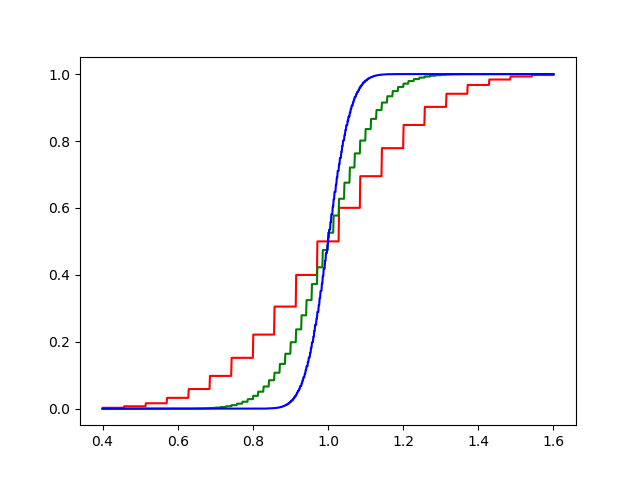
\includegraphics[scale=0.7]{section-06/q6-3.png}
  \end{center}

\end{dinglist}


\begin{enumerate}[(a)]
  \item \q{Que va devenir la fonction de répartition pour un grand nombre de dés ?}
        Elle devient de plus en plus lisse.
        Pour $d$ très grand elle ressemblera à :
        \[
          f(x)=
          \left\{
          \begin{array}{rcl}
            0 & \text{ pour } x<1 \\
            1 & \text{ pour } x>1 \\
          \end{array}
          \right.
        \]

  \item \q{Expliquer ce résultat avec la variance et l’inégalité de Bienaymé-Tchebychev.}
        Inégalité de Bienaymé-Tchebychev :
        \[
          \mathbb{P}(|S_d-E(S_d)| \geq \alpha) \leq \frac{V(S_d)}{\alpha^2}
        \]


\end{enumerate}
